% Section VI: Discussion / Limitations
% All numbers trace to PHASE_B_FINDINGS.md / experiments/out/*.json (see OUTLINE.md §VI).

\section{Discussion and Limitations}
\label{sec:discussion}

\subsection{What the Stitched Density Does and Does Not Buy}
\label{sec:disc-stitch}

\looseness=-1 Table~\ref{tab:seam} is deliberately a parity result. Stitching does
\emph{not} buy nats: a practitioner needing only a rasterized product
loses nothing by cropping. It buys the object itself, a normalized
global density with every fitted component's evidence intact and
duplication resolved by an explicit exact merge, not implicit
deletion. The crop baseline is moreover charitable (globally
renormalized, where deployed pipelines skip it), and deletion's
near-zero cost is an empirical fact of these scenes, not a guarantee:
it grows in principle with the mass straddling seams, a regime this
study does not test. The second site cuts the other way too: SMBU's production
seam bands show a $-0.37$-nat stitched deficit and 68\% seam coverage
of $0.570$ (Secs.~\ref{sec:results:seams}--\ref{sec:results:calibration}),
so neither seam parity nor seam calibration of the stitched rule
travels automatically across sites; both must be checked per campaign.

\subsection{The Level-of-Detection Floor Is Intrinsic}
\label{sec:disc-lod}

\looseness=-1 The change-detection level of detection saturates at approximately
$1.0$~m and no configuration we tried lowers it: the floor survives
the ${\sim}3\times$ capacity increase of Table~\ref{tab:change_dose},
cell sizes 0.5--2~m, and a 2~cm registration term, even as ranking
and precision improve. We conclude it is a representation limit of
Gaussian mixtures on heterogeneous urban vertical structure: roof
edges, facades, and vegetation within one component's support inflate
the posterior mean-location variance the LoD is built from. We
expect no tuning to remove it; sub-meter sensitivity would require a
likelihood modeling vertical layering explicitly. The floor is
consistent with the measured absolute accuracy: model-to-mesh error is
decimeter-grade only in the confident tercile and meter-band in the
worst (Sec.~\ref{sec:results:geoacc}), an order of magnitude above the
centimeter grade classical survey processing achieves on data of this
quality. For the LoD itself the classical yardstick is now measured
(Sec.~\ref{sec:results:change}): the same-grid propagated-error DoD
posts nominal mm--cm thresholds but flags 17--90\% of stable ground,
so the ${\approx}1$~m floor is the price of a held null level here,
not mere bluntness; whether a full M3C2-EP error budget with
explicitly modeled alignment
uncertainty~\cite{winiwarter2021m3c2ep} can hold the null at
centimeter LoDs is the open classical arm (Sec.~\ref{sec:disc-open}).

\subsection{The Density Component of the Uncertainty Signal}
\label{sec:disc-density}

\looseness=-1 As quantified in Sec.~\ref{sec:results:sparsification}, the
predictive-NLPD error ranking is largely internalized sampling
density (a model-free density ranker outranks it, with rank
agreement $\rho = 0.67$--$0.74$), and the within-tercile gain over
random concentrates in the sparsest tercile; the pattern's
replication across a $20\times$ capacity change makes this intrinsic
to the mismatch between LiDAR sampling heteroscedasticity and the
Gaussian observation model, not a resolution artifact. An operator
holding the raw cloud should rank by density; what the predictive
adds is the calibrated, compact form
(Sec.~\ref{sec:results:sparsification}), and its ranking should be
read as ``sparse and poorly explained,'' not as a density-free
model-error signal.

\subsection{What $\hat{K}$ Is and Is Not}
\label{sec:disc-khat}

\looseness=-1 We report the deconfounding of $\hat{K}$ as a finding. On the STPLS3D
matched-$N$ grid (29 scenes $\times$ $\alpha\in\{0.1,1,10\}$ $\times$
2 seeds, all at $N=3\times10^{6}$ points), realized complexity at
$\alpha=1$ falls in the narrow band $\hat{K}\in[18,25]$ from empty
terrain to dense urban, with no content signal:
$\rho(\hat{K},\text{class-entropy})=0.13$ ($p=0.34$),
$\rho(\hat{K},\text{surface variation})=-0.04$,
$\rho(\hat{K},\text{density})=0.00$; the $\alpha=10$ arm is
truncation-pinned at $T=64$, and a prior length-scale sweep (29
scenes $\times$ three scale factors, $0.03$--$0.3\times$ the default,
at $\alpha=1$ and a single seed; the main grid's default-scale arm
supplies the $1\times$ endpoint) leaves per-scene $\hat{K}$ unchanged to
within one component (5 of 29 scenes shift by exactly $\pm1$). In
total 261 controlled fits, the $174$-fit matched-$N$ grid plus the
$87$-fit sweep: under
truncated stick-breaking CAVI at matched $N$, realized complexity is
set by component-death dynamics and data volume, consistent with the
base model's asymptotics~\cite{dong2026dpsplat}; on the H3D tiles,
$\rho(\hat{K},\text{tile point count})=0.97/0.82/0.85$ (full-epoch
reference fits; production refits $0.77$--$0.98$). We claim
$\hat{K}$ only as automatic, data-volume-adaptive capacity
control (useful, since a fixed budget as in
VBGS~\cite{vandemaele2024vbgs} over-provisions empty tiles and starves
dense ones, Fig.~\ref{fig:khat_deconfound}) and disclaim any reading
of $\hat{K}$ as a map of scene content.

\begin{figure}[t]
  \centering
  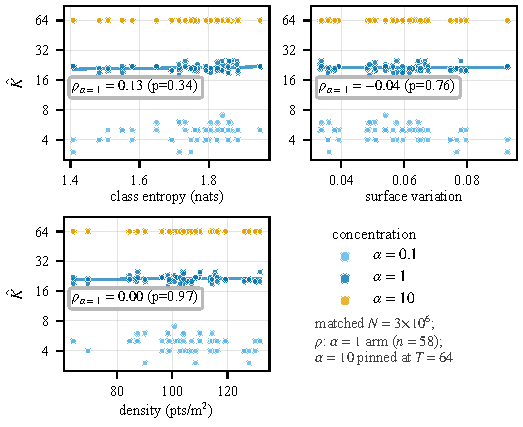
\includegraphics[width=\columnwidth]{figs/stpls3d_khat_vs_complexity.pdf}
  \caption{$\hat{K}$ against scene-content descriptors on the STPLS3D
  matched-$N$ grid (pipeline product; 29 scenes $\times$ 2 seeds per
  concentration arm, annotated $\rho$ and least-squares trend lines
  from the $\alpha{=}1$ arm;
  surface variation is the local-PCA smallest-eigenvalue ratio
  $\lambda_{\min}/\sum_i \lambda_i$ over $k{=}16$ nearest neighbors in
  a fixed $5{\times}10^{4}$-point uniform subsample per scene): the
  association is null, while the $\alpha{=}10$ arm is
  truncation-pinned at $T{=}64$; on real tiled scenes $\hat{K}$
  tracks per-tile point count ($\rho$ up to $0.98$,
  Sec.~\ref{sec:disc-khat}).}
  \label{fig:khat_deconfound}
\end{figure}

\subsection{Scope of the Re-Flight Study}
\label{sec:disc-anchor}

\looseness=-1 The Mill~19 planning results rest on a sparse COLMAP
anchor~\cite{turki2022meganerf}: a planning-scale demonstration on
held-back imagery, with no flights executed and no absolute-scale claims
beyond the anchor's metric coherence. The mass-only control (grant by
pool mass, ignoring the model) has been run in both scenarios
(Sec.~\ref{sec:results:reflight}): the posterior factor is dispensable
for mass-separable grants and demonstrably valuable for
mass-comparable ones; whether that margin persists on dense
photogrammetric products is left to future work
(Sec.~\ref{sec:conclusion}).

\subsection{Open Protocol Questions}
\label{sec:disc-open}

\looseness=-1 Cross-tile merge acceptance is rare at $10^{7}$-point tiles under
$\alpha=1$ (Sec.~\ref{sec:results:seams}), consistent with dominance
of the likelihood term in the sign test at large $N$
(Sec.~\ref{sec:merge}); a halo-width and acceptance-threshold ablation
with an ELBO-based criterion is left to future work, as are
hierarchical Dirichlet-process (HDP) sharing across tiles, a spatially
blocked hold-out
protocol (Sec.~\ref{sec:setup:protocols}), a full M3C2-EP error
budget on the same cells (the plain propagated-error DoD arm is
measured in Sec.~\ref{sec:results:change}), and
external validation of the class-transition change proxy. Finally, we
claim no theoretical seam-coverage guarantee: calibration is an
empirical, per-campaign check
(Secs.~\ref{sec:results:calibration}, \ref{sec:disc-stitch}).
